\section{Конструкторская часть}

% TODO Возможно тексты стоит хранить в виде связного списка предложений, и в аннотациях указывать номер предложения, и начало считать от него.
% Но стоит ли? Может хранить текст просто целиком, и индексироваться по нему абсолютно (int-a хватит для индексирования символов тысячи томов войны и мира в одном файле), а выравнивание хранить в виде отдельной аннотации?
% Думаю лучше создать отдельную таблицу для выровненных фрагментов, чтобы не засорять аннотации выравниванием.

% ПРИМИТИВЫ ВЫРАВНИВАНИЯ
% ----------------------
% - id [PK]
% - тип

% ВЫРАВНИВАНИЕ
% ------------
% - id
% - id текста [FK]
% - id типа [FK]
% - начало
% - конец

\begin{figure}[H]
	\centering
	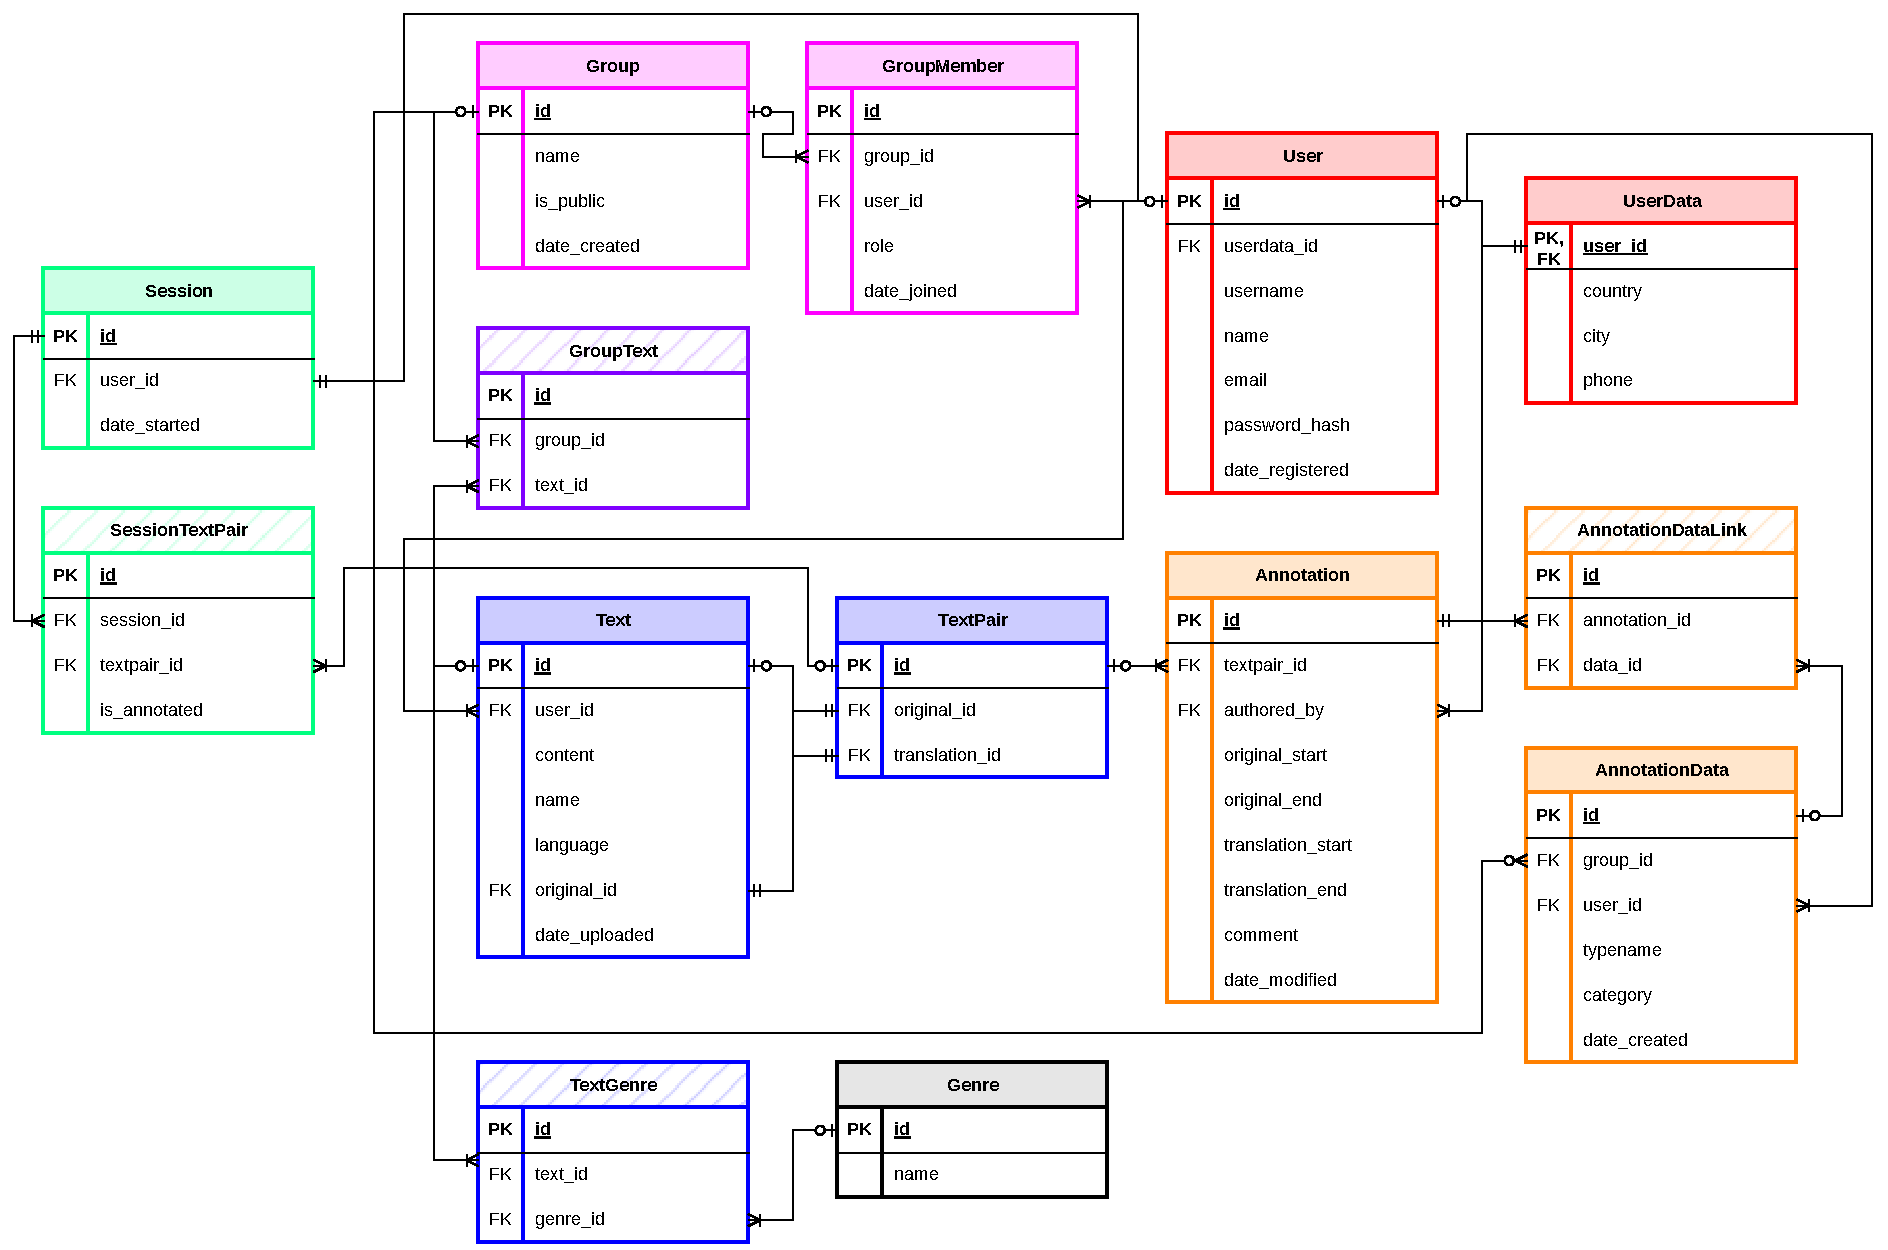
\includegraphics[width=\textwidth]{diag/erd-color.pdf}
	\caption{ER-диаграмма разрабатываемой базы данных}
	\label{fig:erd}
\end{figure}

ERD в нотации Чена: \ref{fig:chen-erd}.


\begin{figure}[H]
	\centering
	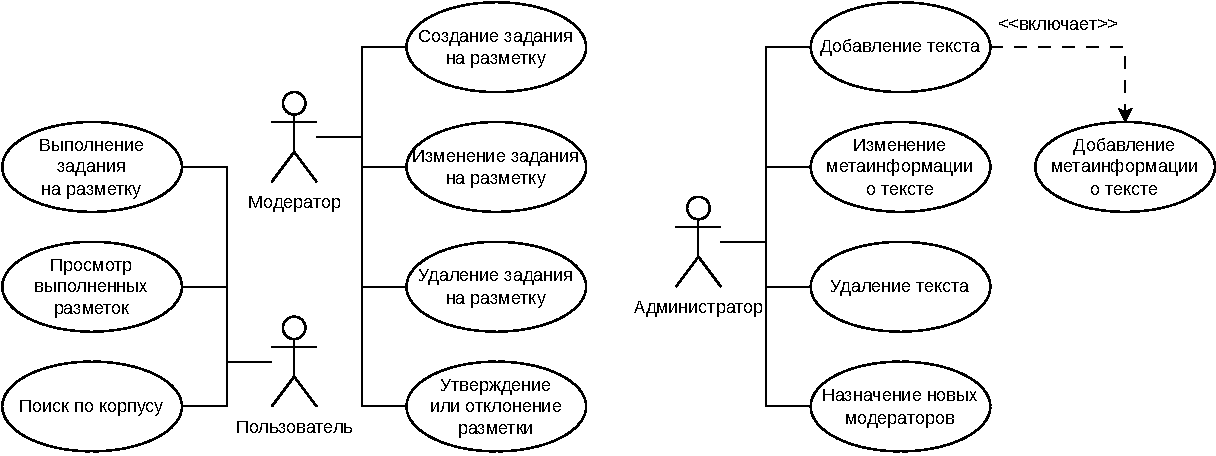
\includegraphics[width=\textwidth]{diag/use-case.pdf}
	\caption{Диаграмма сценария использования}
	\label{fig:use-case}
\end{figure}

\begin{figure}[H]
	\centering
	\includegraphics[width=\textwidth]{diag/auth-bpmn.pdf}
	\caption{Диаграмма процесса аутентификации пользователя}
	\label{fig:auth-bpmn}
\end{figure}

\subsection{Вывод}
